% !TeX root = ..\main.tex

\section{Hazelcast in Practice}
The goal of this section is to test Hazelcast in practice. With this goal in
mind, we will first install Hazelcast, and then we will try to implement some
example data structures. We will take a look at the Usability of the Hazelcast
interface. 

In this section following limitations are taken into account: First only the
Open-Source Hazelcast Platform is used. Second, only the Hazelcast Command Line
Interface (CLI) is used. Therefore, the Hazelcast cloud service Viridian is not
used and will not be evaluated. Furthermore, the Hazelcast Clients outside
the Hazelcast CLI are not used, and will not be evaluated. The data structure
used for testing is taken from a previous lecture.
\todo{}
\subsection{Installation of Hazelcast}
There are multiple ways to install Hazelcast. Due to the fact that Hazelcast is
open-source and provides Binaries. Therefore, it's possible to build the
Hazelcast Platform from source. However, it is easier to download prebuild
binaries. For Linux there is a Debian package available. For macOS there is a
brew package available, but for Windows there is no package or installer
available. Therefore, under Windows you have to download prebuild binaries,
if you don't want to build Hazelcast from source. Another option is to use
docker. \parencite{hazelcast_installing_nodate}

We tried the Hazelcast installation on multiple operating systems, but weren't
able to test the installation on macOS. Therefore, we will only describe the
installation on Linux and Windows, and will take a look at the installation via
docker. The installation on Linux is very easy and straight forward: First you
will download the public key of the Hazelcast repository and add the repository
to your package manager sources:
\begin{lstlisting}[language=bash,caption={Adding the Hazelcast repository to the package manager sources under Linux (Debian) \parencite{hazelcast_installing_nodate}}]
wget -qO - https://repository.hazelcast.com/api/gpg/key/public | gpg --dearmor | sudo tee /usr/share/keyrings/hazelcast-archive-keyring.gpg > /dev/null
echo "deb [signed-by=/usr/share/keyrings/hazelcast-archive-keyring.gpg] https://repository.hazelcast.com/debian stable main" | sudo tee -a /etc/apt/sources.list
\end{lstlisting}
After that you will be able to install Hazelcast via the package manager like
any other package:
\begin{lstlisting}[language=bash,caption={Installing Hazelcast under Linux (Debian) \parencite{hazelcast_installing_nodate}}]
sudo apt update && sudo apt install hazelcast
\end{lstlisting}
The installation under Windows was a bit more complicated. First
Hazelcast did not provide a Windows installer. Therefore, we had to download the
binary from the Hazelcast website. This binary wasn't able to run directly,
because it needed the \texttt{JAVA\_HOME} environment variable to be set. First we
tried to install a Java Runtime Environment (JRE) and set the \texttt{JAVA\_HOME}
variable accordingly. However, the JRE was not able to run the Hazelcast binary
and a Java Development Kit (JDK) was needed. Therefore, we installed the JDK set
the path, and then the Hazelcast binary was able to run. However, personally we
found the installation with docker the easiest. 
First, the Hazelcast image is downloaded from the docker hub:
\begin{lstlisting}[language=bash,caption={Downloading the Hazelcast image from the docker hub \parencite{hazelcast_installing_nodate}}]
docker pull hazelcast/hazelcast
\end{lstlisting}
After that the local Hazelcast Cluster is started as specified in the
documentation:
\begin{lstlisting}[language=bash,caption={Starting the Hazelcast Cluster using the docker image \parencite{hazelcast_start_2023}}]
docker network create hazelcast-network
docker run \
    -it \
    --network hazelcast-network \
    --rm \
    -e HZ_CLUSTERNAME=hello-world \
    -p 5701:5701 hazelcast/hazelcast
\end{lstlisting}

For the following example the docker installation will be used. 

\subsection{Example in Hazelcast}
In this section an example data structure will be implemented using the Hazelcast
CLI. The Hazelcast CLI is run as a docker container. 
The data structure is taken from a previous lecture and shown in
\cref{fig:datastructure}.
\begin{figure}[h]
    \centering
    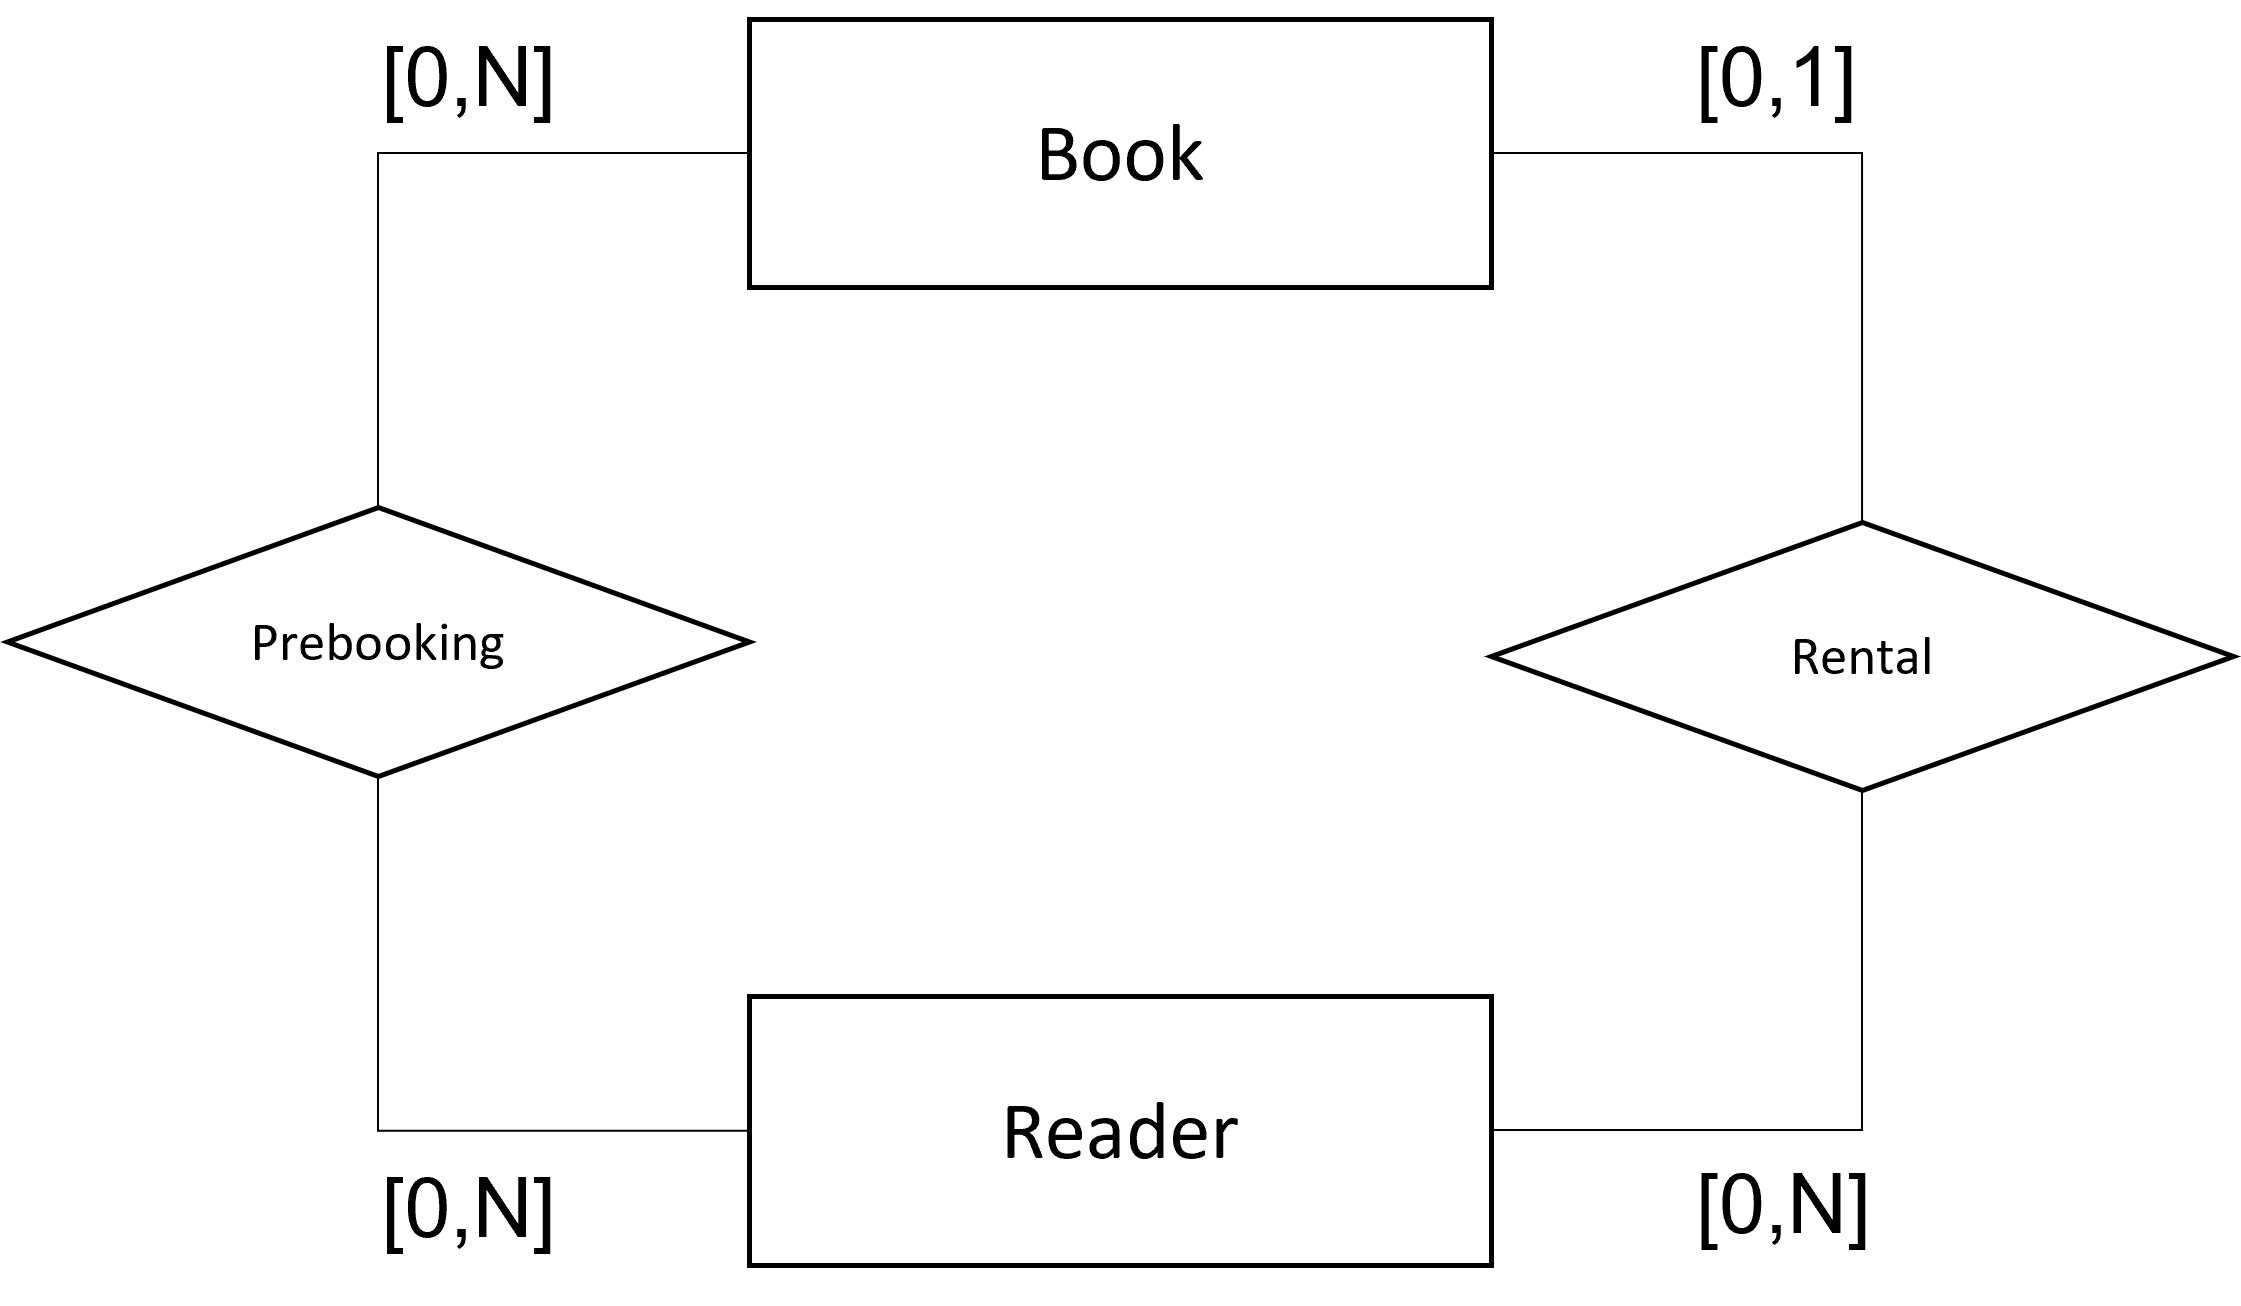
\includegraphics[width=.5\linewidth]{images/Datastructure.png}
    \caption{Example data structure \parencite[see also][]{mairhofer_aufgabe_2021}}
    \label{fig:datastructure}
\end{figure}
The data structure models a library with books. The library has multiple books
and multiple readers. Each book can be rented by one reader. The reader can rent
multiple books. And if a book is rented by a reader, another reader can't rent
it, but order a prebooking for it. This data structure was given to us in an
example in a previous lecture by \textcite{mairhofer_aufgabe_2021}. The exact
fields of the data structure are not important for this example. The important
part is that the data structure requires foreign keys to model the relations.

Hazelcast is a distributed key-value store, as described in
\cref{sec:hazelcast-in-theory}. It does not provide a relational database, and it
has no support for foreign keys. It is possible to implement relations with
embedded objects or with user defined fields. To define the Relations between
the object classes we will use user defined fields. Embedded objects have the
problem, that there are hard to manage by hand and difficult to implement
many-to-many relations. In the user defined fields we can define the fields like
a foreign key in a relational database, but Hazelcast does not provide any
safety checks. Therefore, a user has to implement safety checks by hand, if the
consistency in the relations are important. In this example we will not write an
application and only take a look at the Hazelcast CLI. Therefore, we will not
implement any safety checks. But Hazelcast provides a way to select and join
different maps. Thus, it is possible to implement the relations and query those
relations inside the Hazelcast CLI. 

To conclude our example we have successfully implemented a data structure with
foreign keys in the key-value store Hazelcast. However, the relations are not
checked by the Hazelcast platform and the user has to implement the checks to
ensure that the relations are consistent. Therefore, we advise using Hazelcast
as a key-value store and not to try using the Hazelcast platform to implement
complex relations. 